\chapter{Analysis} \label{Analysis}

%Summary: describe how we get real numbers to put into previous part
%Goal: define and obtain real numbers from the previous part
\section{Benchmarks}
Discussion of benchmarks (show size vs resources) FFT, PFB,

\begin{figure}[ht!]
  \centering
    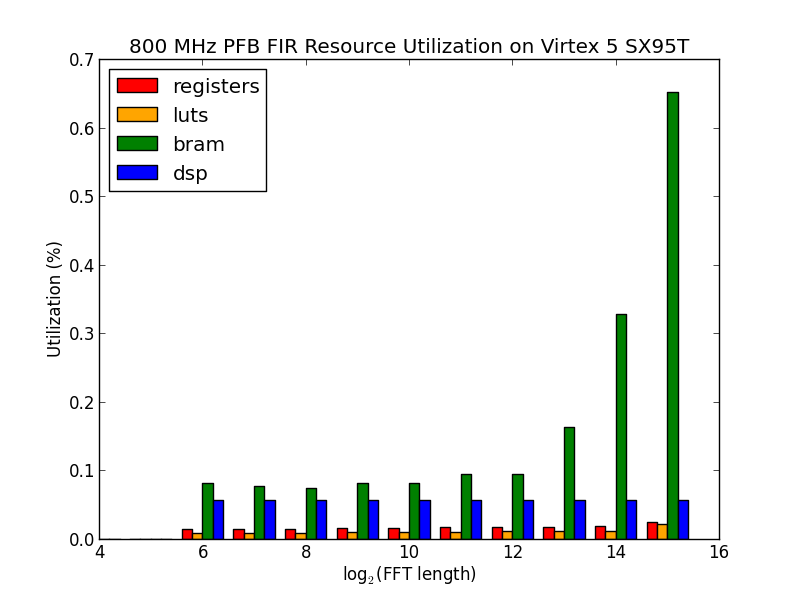
\includegraphics[width=0.49\textwidth]{Images/C6/pfb_bench.png}
  \caption{TODO}
  \label{fig: C6/pfb_bench.png}
\end{figure}

\begin{figure}[ht!]
  \centering
    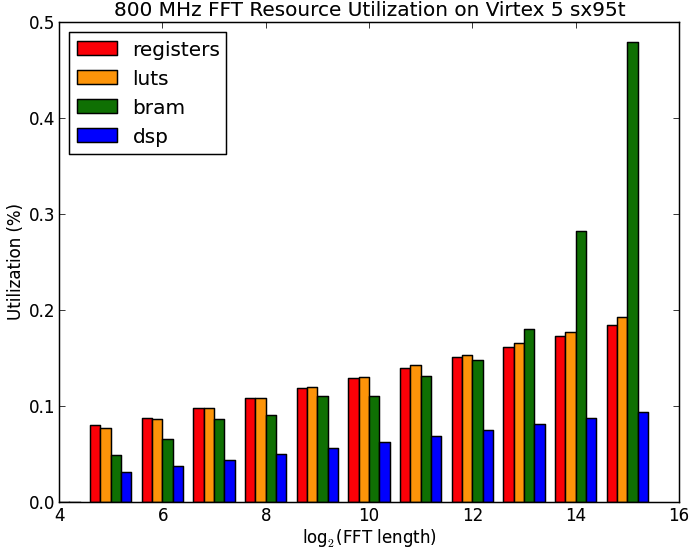
\includegraphics[width=0.49\textwidth]{Images/C6/fft_bench.png}
    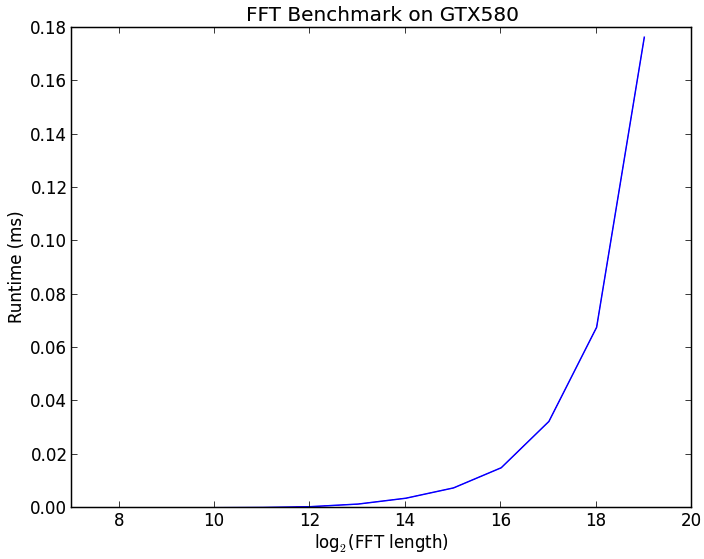
\includegraphics[width=0.49\textwidth]{Images/C6/fft_gpu_bench.png}
  \caption{TODO}
  \label{fig: C6/fft_bench.png}
\end{figure}

refer to casper fft model paper

refer to xgpu paper

%Summary: case studies describing partitioning of realistic-scale instruments
%Goal: show successful application of tool to design of realistic instruments
%provide analysis comparing this to hand-designed instruments 
\section{Simple spectrometer}
Simple spectrometer placement
Include appropriate FFT or PFB benchmarks
\subsection{Cost}
\subsection{Power}

\section{Hi res spectrometer}
results for hi res spectrometer (gbt and seti)
Same benchmarks as before, just discuss large bw, multi stage fft
\subsection{Cost}
\subsection{Power}

\section{Pulsar processor}
extend to pulsar processor design
Need benchmarks for deconvolution algorithm (just cpu vs gpu? infeasible in fpga...) bug jonathon about this
\subsection{Cost}
\subsection{Power}

\section{Cross-correlator}
xgpu benchmarks, correlator placement
Need benchmarks for xengine
\subsection{Cost}
\subsection{Power}
